\chapter{\IfLanguageName{dutch}{POC: Simulatie}{POC: Simulation}}%
\label{ch:poc}

\section{\IfLanguageName{dutch}{Simulatie}{Simulation}}%
\label{sec:sim}%
De \gls{poc} is een simulatie van een 5G-netwerk. Dit wordt opgezet door gebruik te maken van \gls{open5gs} en \gls{ueransim}. De \gls{vm} met als \gls{os} Ubuntu, versie 22.04.5 LTS ook wel gekend als Jammy. 

De opbouw van de simulatie zal in 2 fases gebeuren. \\De eerste is een volledig manuele build. Hier wordt een 5G-netwerk gesimuleerd op een laptop. Dit netwerk bestaat uit een 5G core server en een 5G RAN server. In de simulatie zal de 5G Core server \gls{open5gs} en de 5G RAN server van UERANSIM draaien als simulatie software. Op de 5 RAN Server zijn op zich nog 2 deel elementen aanwezig die verbinden met het netwerk \gls{gnb} en een \gls{ue}. De 2de fase is het omzetten van deze manuele build naar een automatische deployment van de \gls{poc}. Hieronder is een schematische weergaven van de opstelling in de simulatie. 

\begin{figure}[H]
    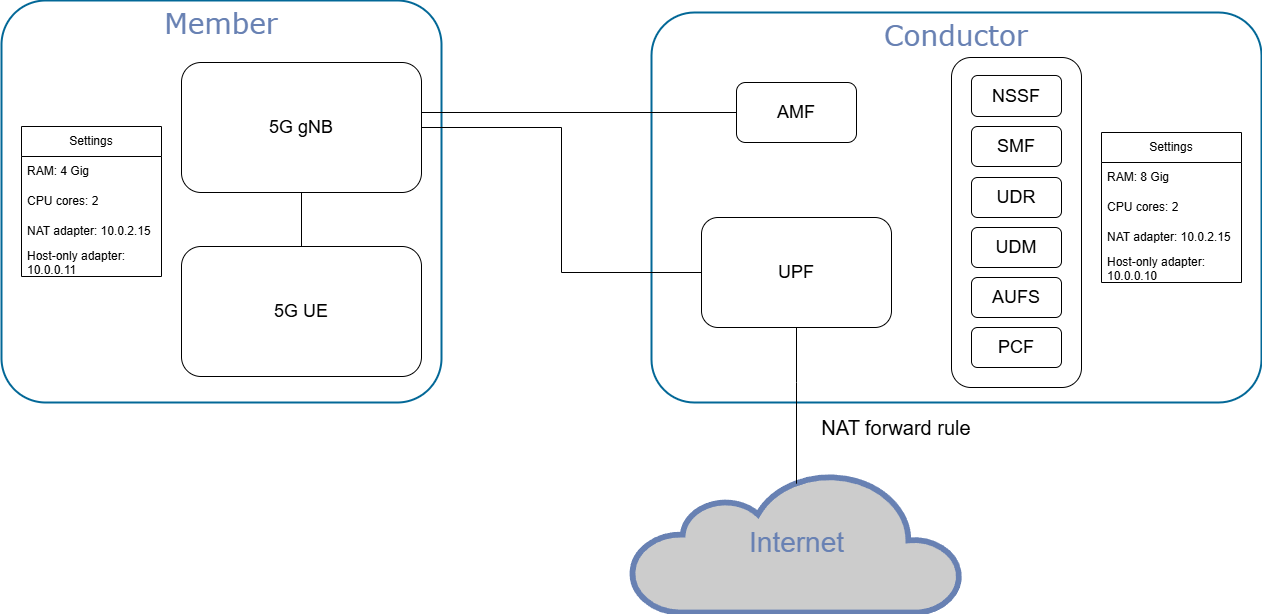
\includegraphics[width=\linewidth]{../graphics/POC-setup.png}
    \caption{POC Set-up (Illustratie)}
    \label{fig:poc-setup}
\end{figure}

Voor de hardware configuratie is er voor de volgende set-up gekozen:

\begin{table}[H]
\centering
\begin{tabular}{|l|l|l|}
\hline
\textbf{Harware configuratie} & \textbf{5G core server} & \textbf{5G RAN server} \\
\hline
RAM & 8 Gigabyte & 4 Gigabyte \\
CPU-cores & 2 & 2 \\
Netwerkkaart & \begin{tabular}[c]{@{}l@{}}NAT (VirtualBox)\\ Host-only, static IP 10.0.0.10\end{tabular} & \begin{tabular}[c]{@{}l@{}}NAT (VirtualBox)\\ Host-only, static IP 10.0.0.11\end{tabular} \\
\hline
\end{tabular}
\caption{Configuratie van 5G core en RAN servers}
\end{table}

% \textbf{5G core server}:
% \begin{itemize}
%     \item RAM: 8 Gigabyte
%     \item CPU-cores: 2
%     \item Netwerkkaart
%     \subitem NAT (VirtualBox)
%     \subitem Host-only met static IP 10.0.0.10
% \end{itemize}

% \textbf{5G RAN server}:
% \begin{itemize}
%     \item RAM: 4 Gigabyte
%     \item CPU-cores: 2
%     \item Netwerkkaart
%     \subitem NAT (VirtualBox)
%     \subitem Host-only met static IP 10.0.0.11
% \end{itemize}

\section{\IfLanguageName{dutch}{Installatie}{Installation}}%
\label{sec:installation}%

De installatie bestaat uit 3 delen:

\begin{itemize}
    \item Vereiste software
    \item Open5GS
    \item UERANSIM
\end{itemize}

De basis installatie van Open5GS gebeurt volgens de Quickstart van \gls{open5gs}, \textcite{Lee2025a} en wordt enkel uitgevoerd op de 5G Core Server (of Conductor \gls{vm}):

\begin{enumerate}
    \item Installatie van afhankelijkheden/vereisten
    \item Installatie van \gls{open5gs}
    \item Configuratie van \gls{open5gs}
    \item Starten van de \gls{open5gs} services
\end{enumerate}

Vervolgens wordt op de 2de \gls{vm}, ook wel de Member \gls{vm} genoemd, \gls{ueransim} geïnstalleerd om de installatiefase te finaliseren. 

De volledige installatie gids is ook toegevoegd in de bijlagen, zie bijlage \ref{ch:InstallationGuide}.\\

Er zijn ook eigen configuratie aanpassingen gebeurt om deze \gls{poc} automatisch te deployen via Vagrant. Hiervoor is er gebruikgemaakt van een Vagrantfile. Deze bevat de hardware configuratie en een link naar het installatie script voor de simulatie. De Vagrantfile is samen met de installatiescripten toegevoegd aan de bijlagen (zie Bijlagen \ref{ch:InstallationGuide} en \ref{ch:vagrant}). Echter sommige configuratie aanpassingen moeten nog steeds manueel worden uitgevoerd, deze wordt verduidelijkt verder in dit hoofdstuk.\\
Om deze \gls{vm} te maken wordt er gebruikgemaakt van het commando: \lstinline!vagrant up!. Echter door het meermaals testen van de \gls{vm} is er gekozen om een script te schrijven in powershell. Dit script verwijdert de vorige \gls{vm} en start de logging van de terminal. Dit is handig om te detecteren of de \gls{vm} klaar is met de configuratie, maar ook om mogelijk fouten sneller te detecteren.

\begin{lstlisting}[basicstyle=\small, frame=single, breaklines=true, postbreak=\mbox{\textcolor{red}{$\hookrightarrow$}\space}, escapeinside ={\%,}, escapechar={!}, numbers=left, language=sh, caption=Build Script]
Start-Transcript -Path "vagrant.log"
vagrant destroy -f
vagrant up
Stop-Transcript
\end{lstlisting}

\section{\IfLanguageName{dutch}{Configuratie}{Configuration}}%
\label{sec:Config}%

De automatische configuratie wordt gedeployd door het oproepen van een script. Dit is geschreven in bash voor Linux, terug te vinden in de bijlagen (Bijlage \ref{ch:vagrant}).\\

Het einde van de automatische configuratie kan worden gedetecteerd aan de hand van de log file die wordt gegenereerd tijdens de installatie in de github-repopository. Deze log file, vagrant.log, is beschikbaar door de shared folder die wordt aangemaakt in het begin van de \gls{vm} installatie. \\

Eenmaal de configuratie klaar is moet enkel de handmatige configuratie gebeuren.
Om te verbinden met de \gls{vm} kan er gebruik worden gemaakt van het 'vagrant ssh' commando.

De manuale configuratie bestaat uit 4 delen:

\begin{itemize}
    \item IP check
    \item Open5GS \gls{amf} configuratie
    \item Open5GS \gls{upf} configuratie
    \item UE configuratie
    \item gNB configuratie
\end{itemize}

Eerst wordt er gekeken naar de huidige IP van de \gls{vm}'s, dit via het \lstinline!ip a! commando. Hier kan men het IP adres van de netwerkkaar eth1. Deze IP adres zullen worden gebruikt voor verdere configuratie. In het geval van de\gls{poc}, is dit 10.0.0.10 en 10.0.0.11

\begin{lstlisting}[basicstyle=\small, frame=single, breaklines=true, postbreak=\mbox{\textcolor{red}{$\hookrightarrow$}\space}, escapeinside ={\%,}, escapechar={!}, numbers=left, language=sh, caption=IP configuratie Centrale]
vagrant@Centrale:~$ ip a
1: lo: <LOOPBACK,UP,LOWER_UP> mtu 65536 qdisc noqueue state UNKNOWN group default qlen 1000
    link/loopback 00:00:00:00:00:00 brd 00:00:00:00:00:00
    inet 127.0.0.1/8 scope host lo
       valid_lft forever preferred_lft forever
    inet6 ::1/128 scope host noprefixroute
       valid_lft forever preferred_lft forever
2: eth0: <BROADCAST,MULTICAST,UP,LOWER_UP> mtu 1500 qdisc fq_codel state UP group default qlen 1000
    link/ether 08:00:27:e1:3d:ae brd ff:ff:ff:ff:ff:ff
    altname enp0s3
    inet 10.0.2.15/24 metric 100 brd 10.0.2.255 scope global dynamic eth0
       valid_lft 75360sec preferred_lft 75360sec
    inet6 fe80::a00:27ff:fee1:3dae/64 scope link
       valid_lft forever preferred_lft forever
3: eth1: <BROADCAST,MULTICAST,UP,LOWER_UP> mtu 1500 qdisc fq_codel state UP group default qlen 1000
    link/ether 08:00:27:77:a3:88 brd ff:ff:ff:ff:ff:ff
    altname enp0s8
    inet 10.0.0.10/24 brd 10.0.0.255 scope global eth1
       valid_lft forever preferred_lft forever
    inet6 fe80::a00:27ff:fe77:a388/64 scope link
       valid_lft forever preferred_lft forever
4: ogstun: <POINTOPOINT,MULTICAST,NOARP,UP,LOWER_UP> mtu 1400 qdisc fq_codel state UP group default qlen 500
    link/none
    inet 10.45.0.1/16 brd 10.45.255.255 scope global ogstun
       valid_lft forever preferred_lft forever
    inet6 2001:db8:cafe::1/48 scope global
       valid_lft forever preferred_lft forever
    inet6 fe80::374e:8270:9762:52a6/64 scope link stable-privacy
       valid_lft forever preferred_lft forever
\end{lstlisting}

\begin{lstlisting}[basicstyle=\small, frame=single, breaklines=true, postbreak=\mbox{\textcolor{red}{$\hookrightarrow$}\space}, escapeinside ={\%,}, escapechar={!}, numbers=left, language=sh, caption=IP configuratie Member]
vagrant@ue:~$ ip a
1: lo: <LOOPBACK,UP,LOWER_UP> mtu 65536 qdisc noqueue state UNKNOWN group default qlen 1000
    link/loopback 00:00:00:00:00:00 brd 00:00:00:00:00:00
    inet 127.0.0.1/8 scope host lo
       valid_lft forever preferred_lft forever
    inet6 ::1/128 scope host noprefixroute
       valid_lft forever preferred_lft forever
2: eth0: <BROADCAST,MULTICAST,UP,LOWER_UP> mtu 1500 qdisc fq_codel state UP group default qlen 1000
    link/ether 08:00:27:e1:3d:ae brd ff:ff:ff:ff:ff:ff
    altname enp0s3
    inet 10.0.2.15/24 metric 100 brd 10.0.2.255 scope global dynamic eth0
       valid_lft 76464sec preferred_lft 76464sec
    inet6 fe80::a00:27ff:fee1:3dae/64 scope link
       valid_lft forever preferred_lft forever
3: eth1: <BROADCAST,MULTICAST,UP,LOWER_UP> mtu 1500 qdisc fq_codel state UP group default qlen 1000
    link/ether 08:00:27:d2:32:c5 brd ff:ff:ff:ff:ff:ff
    altname enp0s8
    inet 10.0.0.11/24 brd 10.0.0.255 scope global eth1
       valid_lft forever preferred_lft forever
    inet6 fe80::a00:27ff:fed2:32c5/64 scope link
       valid_lft forever preferred_lft forever
\end{lstlisting}

\subsection{\IfLanguageName{dutch}{Open5GS AMF en UPF configuratie}{Open5GS AMF and UPF configuration}}%
\label{sec:open5gs_amf-upf}%

Eenmaal het IP adres gekend is worden de hierboven opgelijste configuraties aangepast, beginnend met de \gls{amf}. Hierbij wordt op lijn 23 het ip adres 127.0.0.5 naar het gevonden ip adres 10.0.0.10. Dit is het IP adres van de ngap server.

\begin{lstlisting}[basicstyle=\small, frame=single, breaklines=true, postbreak=\mbox{\textcolor{red}{$\hookrightarrow$}\space}, escapeinside ={\%,}, escapechar={!}, numbers=left, language=sh, caption=Open5GS amf configuratie]
logger:
    file:
        path: /var/log/open5gs/amf.log
#  level: info   # fatal|error|warn|info(default)|debug|trace

global:
    max:
        ue: 1024  # The number of UE can be increased depending on memory size.
#    peer: 64

amf:
    sbi:
        server:
            - address: 127.0.0.5
            port: 7777
        client:
#      nrf:
#        - uri: http://127.0.0.10:7777
        scp:
            - uri: http://127.0.0.200:7777
    ngap:
        server:
            - address: 10.0.0.10  #CHANGED VALUE
...
\end{lstlisting}

Vervolgens wordt de configuratie van \gls{upf} aangepast op lijn 20. Hier wordt het adres van de gtpu server aangepast naar die van de 5G Core server.

\begin{lstlisting}[basicstyle=\small, frame=single, breaklines=true, postbreak=\mbox{\textcolor{red}{$\hookrightarrow$}\space}, escapeinside ={\%,}, escapechar={!}, numbers=left, language=sh, caption=Open5GS upf configuratie]
logger:
  file:
    path: /var/log/open5gs/upf.log
#  level: info   # fatal|error|warn|info(default)|debug|trace

global:
  max:
    ue: 1024  # The number of UE can be increased depending on memory size.
#    peer: 64

upf:
  pfcp:
    server:
      - address: 127.0.0.7
    client:
#      smf:     #  UPF PFCP Client try to associate SMF PFCP Server
#        - address: 127.0.0.4
  gtpu:
    server:
      - address: 10.0.0.10  #CHANGED VALUE
  session:
    - subnet: 10.45.0.0/16
      gateway: 10.45.0.1
    - subnet: 2001:db8:cafe::/48
      gateway: 2001:db8:cafe::1
  metrics:
    server:
      - address: 127.0.0.7
        port: 9090
...
\end{lstlisting}

Het is heel belangrijk om de \gls{amf} en \gls{upf} te herstarten om de nieuwe configuaratie in te laden. Dit wordt gedaan met het commando: 

\begin{lstlisting}[basicstyle=\small, frame=single, breaklines=true, postbreak=\mbox{\textcolor{red}{$\hookrightarrow$}\space}, escapeinside ={\%,}, escapechar={!}, numbers=left, language=sh, caption=Reload AMF en UPF]
sudo systemctl daemon-reload
sudo systemctl restart open5gs-amfd
sudo systemctl restart open5gs-upfd
\end{lstlisting}

\subsection{\IfLanguageName{dutch}{gNB configuratie}{gNB configuration}}%
\label{sec:gnb_config}%

\begin{lstlisting}[basicstyle=\small, frame=single, breaklines=true, postbreak=\mbox{\textcolor{red}{$\hookrightarrow$}\space}, escapeinside ={\%,}, escapechar={!}, numbers=left, language=sh, caption=gnb configuratie]
mcc: '999'          # Mobile Country Code value
mnc: '70'           # Mobile Network Code value (2 or 3 digits)

nci: '0x000000010'  # NR Cell Identity (36-bit)
idLength: 32        # NR gNB ID length in bits [22...32]
tac: 1              # Tracking Area Code

linkIp: 10.0.0.11 #CHANGED VALUE   # gNB's local IP address for Radio Link Simulation (Usually same with local IP)
ngapIp: 10.0.0.11 #CHANGED VALUE  # gNB's local IP address for N2 Interface (Usually same with local IP)
gtpIp: 10.0.0.11 #CHANGED VALUE    # gNB's local IP address for N3 Interface (Usually same with local IP)

# List of AMF address information
amfConfigs:
    - address: 10.0.0.10 #CHANGED VALUE
        port: 38412

# List of supported S-NSSAIs by this gNB
slices:
    - sst: 1

# Indicates whether or not SCTP stream number errors should be ignored.
ignoreStreamIds: true
\end{lstlisting}

\subsection{\IfLanguageName{dutch}{UE configuratie}{UE configuration}}%
\label{sec:ue_config}%

\begin{lstlisting}[basicstyle=\small, frame=single, breaklines=true, postbreak=\mbox{\textcolor{red}{$\hookrightarrow$}\space}, escapeinside ={\%,}, escapechar={!}, numbers=left, language=sh, caption=UE configuratie]
# IMSI number of the UE. IMSI = [MCC|MNC|MSISDN] (In total 15 digits)
supi: 'imsi-999700000000001'
# Mobile Country Code value of HPLMN
mcc: '999'
# Mobile Network Code value of HPLMN (2 or 3 digits)
mnc: '70'
# SUCI Protection Scheme : 0 for Null-scheme, 1 for Profile A and 2 for Profile B
protectionScheme: 0
# Home Network Public Key for protecting with SUCI Profile A
homeNetworkPublicKey: '5a8d38864820197c3394b92613b20b91633cbd897119273bf8e4a6f4eec0a650'
# Home Network Public Key ID for protecting with SUCI Profile A
homeNetworkPublicKeyId: 1
# Routing Indicator
routingIndicator: '0000'

# Permanent subscription key
key: '465B5CE8B199B49FAA5F0A2EE238A6BC'
# Operator code (OP or OPC) of the UE
op: 'E8ED289DEBA952E4283B54E88E6183CA'
# This value specifies the OP type and it can be either 'OP' or 'OPC'
opType: 'OPC'
# Authentication Management Field (AMF) value
amf: '8000'
# IMEI number of the device. It is used if no SUPI is provided
imei: '356938035643803'
# IMEISV number of the device. It is used if no SUPI and IMEI is provided
imeiSv: '4370816125816151'

# Network mask used for the UE's TUN interface to define the subnet size
tunNetmask: '255.255.255.0'

# List of gNB IP addresses for Radio Link Simulation
gnbSearchList:
    - 10.0.0.11 #CHANGED VALUE

...
\end{lstlisting}

\subsection{\IfLanguageName{dutch}{Subscriber configuratie}{Subscriber configuration}}%
\label{sec:subscriber_config}%

Voor de configuratie van de subscriber moet er gebruik gemaakt worden van de \gls{open5gs} Web interface. Hiervoor is er een forward-regel zodat deze via de browser van de host-laptop kan worden geraadpleegd op 'localhost:9999'. Dan wordt de gebruiker verwelkomd met dit aanmeldscherm:

\begin{figure}[H]
    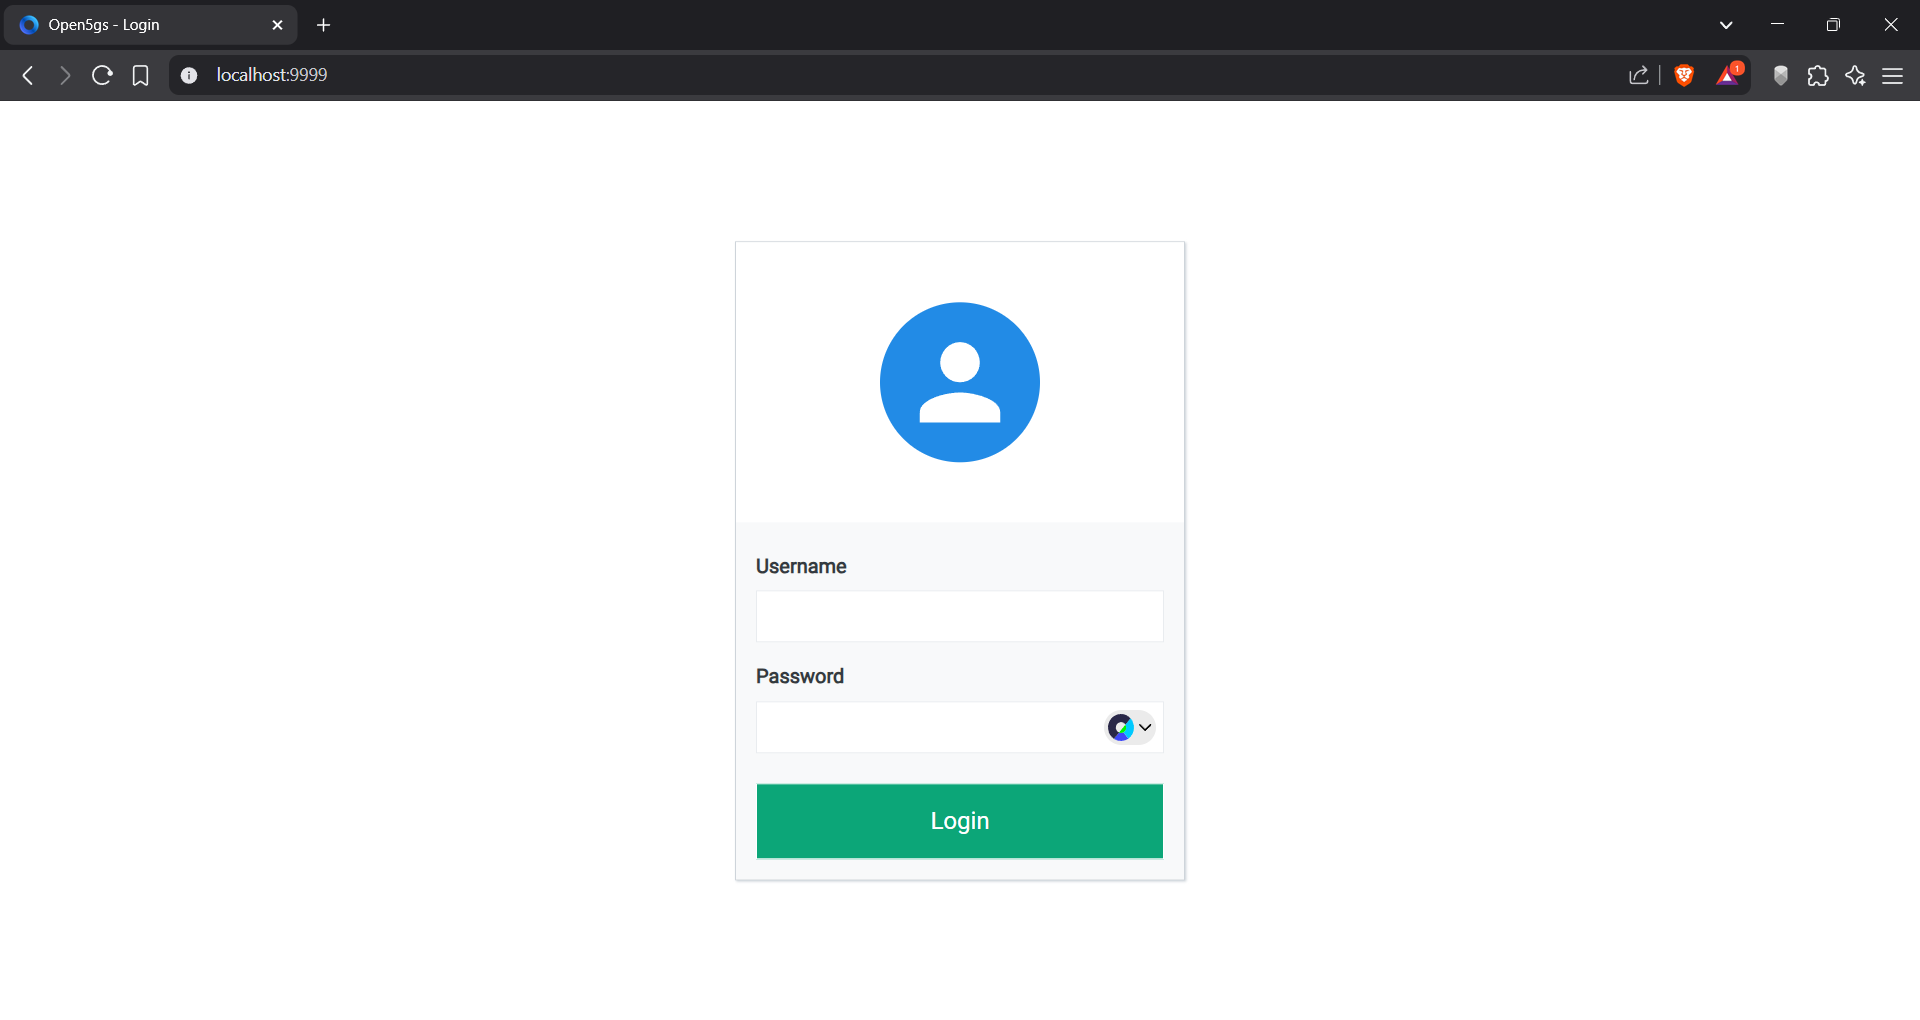
\includegraphics[width=\linewidth]{../graphics/POC-WebUI-Login.png}
    \caption{Aanmeldscherm Open5GS WebUI (Screenshot)}
    \label{fig:Aanmeld WebUI}
\end{figure}

Eenmaal aangemeld met de correcte gegevens, terug te vinden in de config-files:

\begin{itemize}
    \item Username: admin
    \item Password: 1423
\end{itemize}

\begin{figure}[H]
    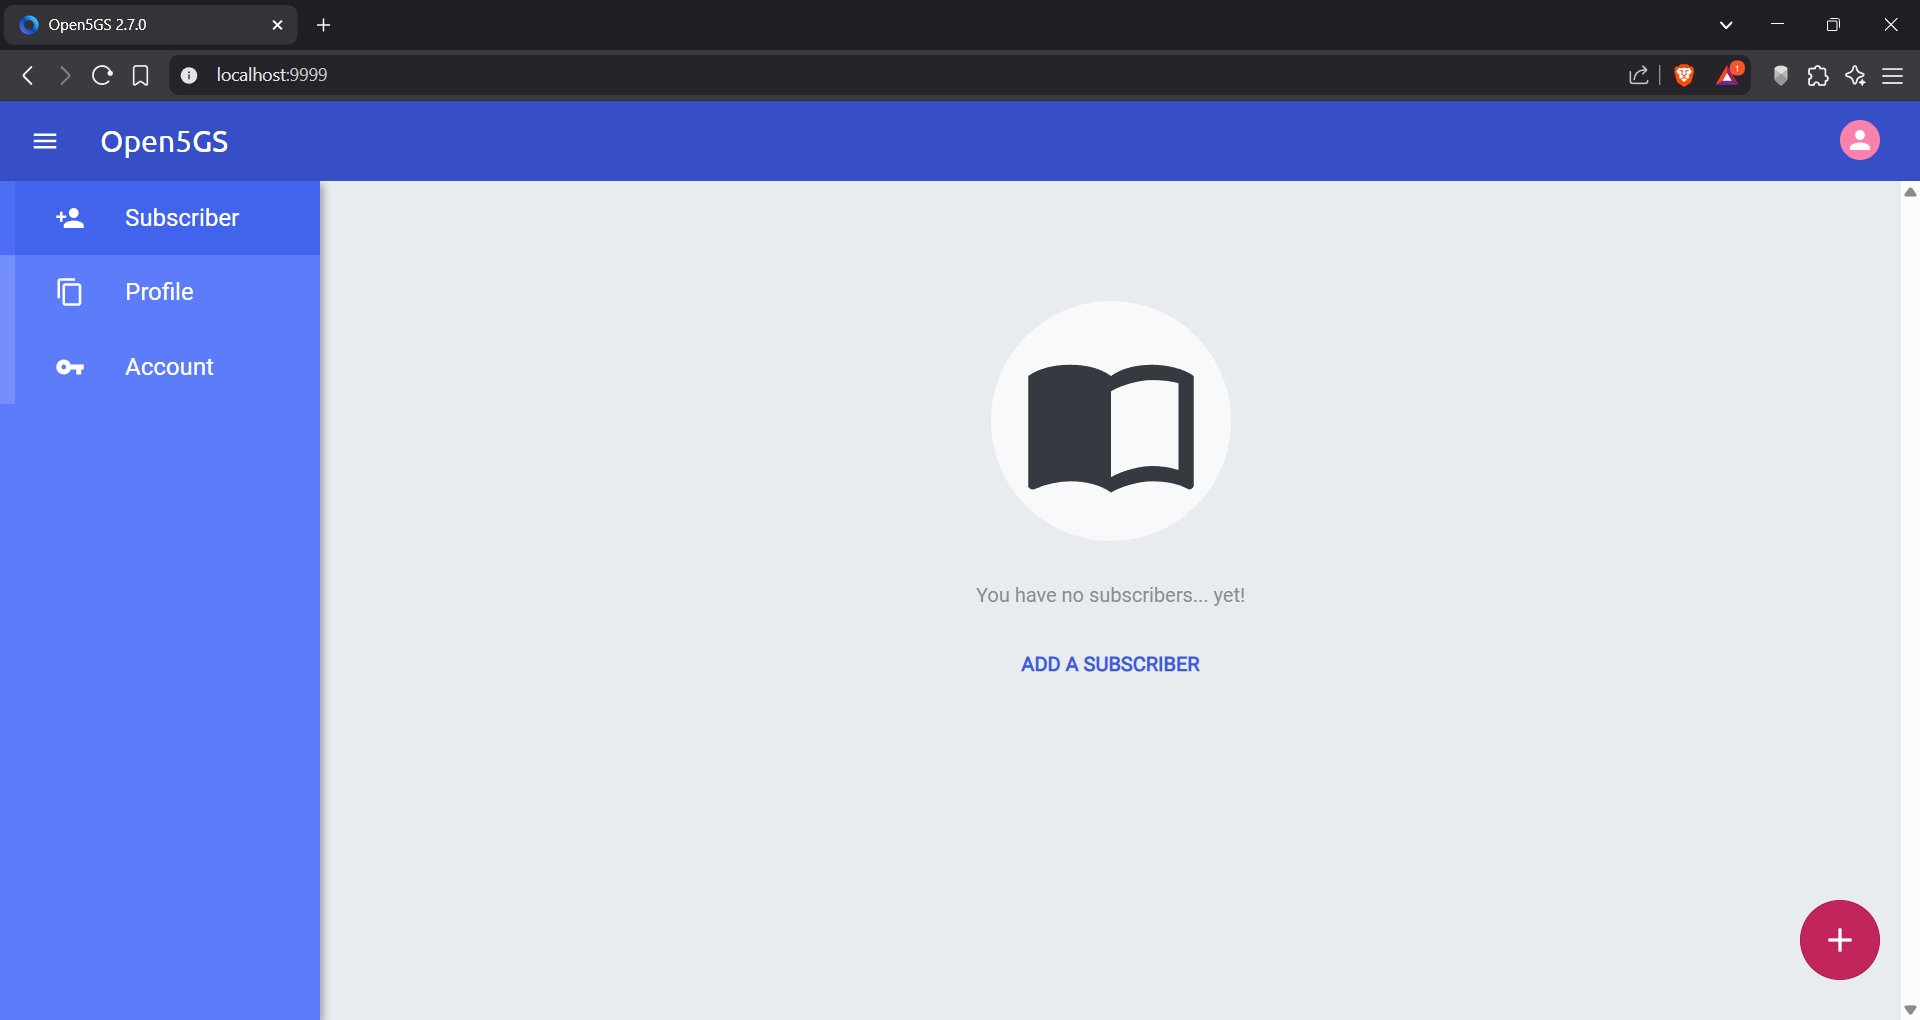
\includegraphics[width=\linewidth]{../graphics/POC-WebUI-home.png}
    \caption{Homescherm Open5GS WebUI (Screenshot)}
    \label{fig:Home WebUI}
\end{figure}

Nadien kan een  subscriber worden toegevoegd.
Voor de feitelijke configuratie van de subscriber zijn er gegevens nodig uit de configuaratie file van de \gls{ue}. De gegevens die nodig zijn:

\begin{itemize}
    \item \gls{imsi}
    \item Subscriber Key
    \item \gls{amf}
    \item USIM Type
    \item Operator Key
\end{itemize}

Deze gegevens worden retchstreeks overgenomen uit de configuratie file naar de webinterface voor \gls{open5gs}. Hier kunnen meerdere toestellen als \gls{ue} worden geregistreerd. 
\begin{figure}[H]
    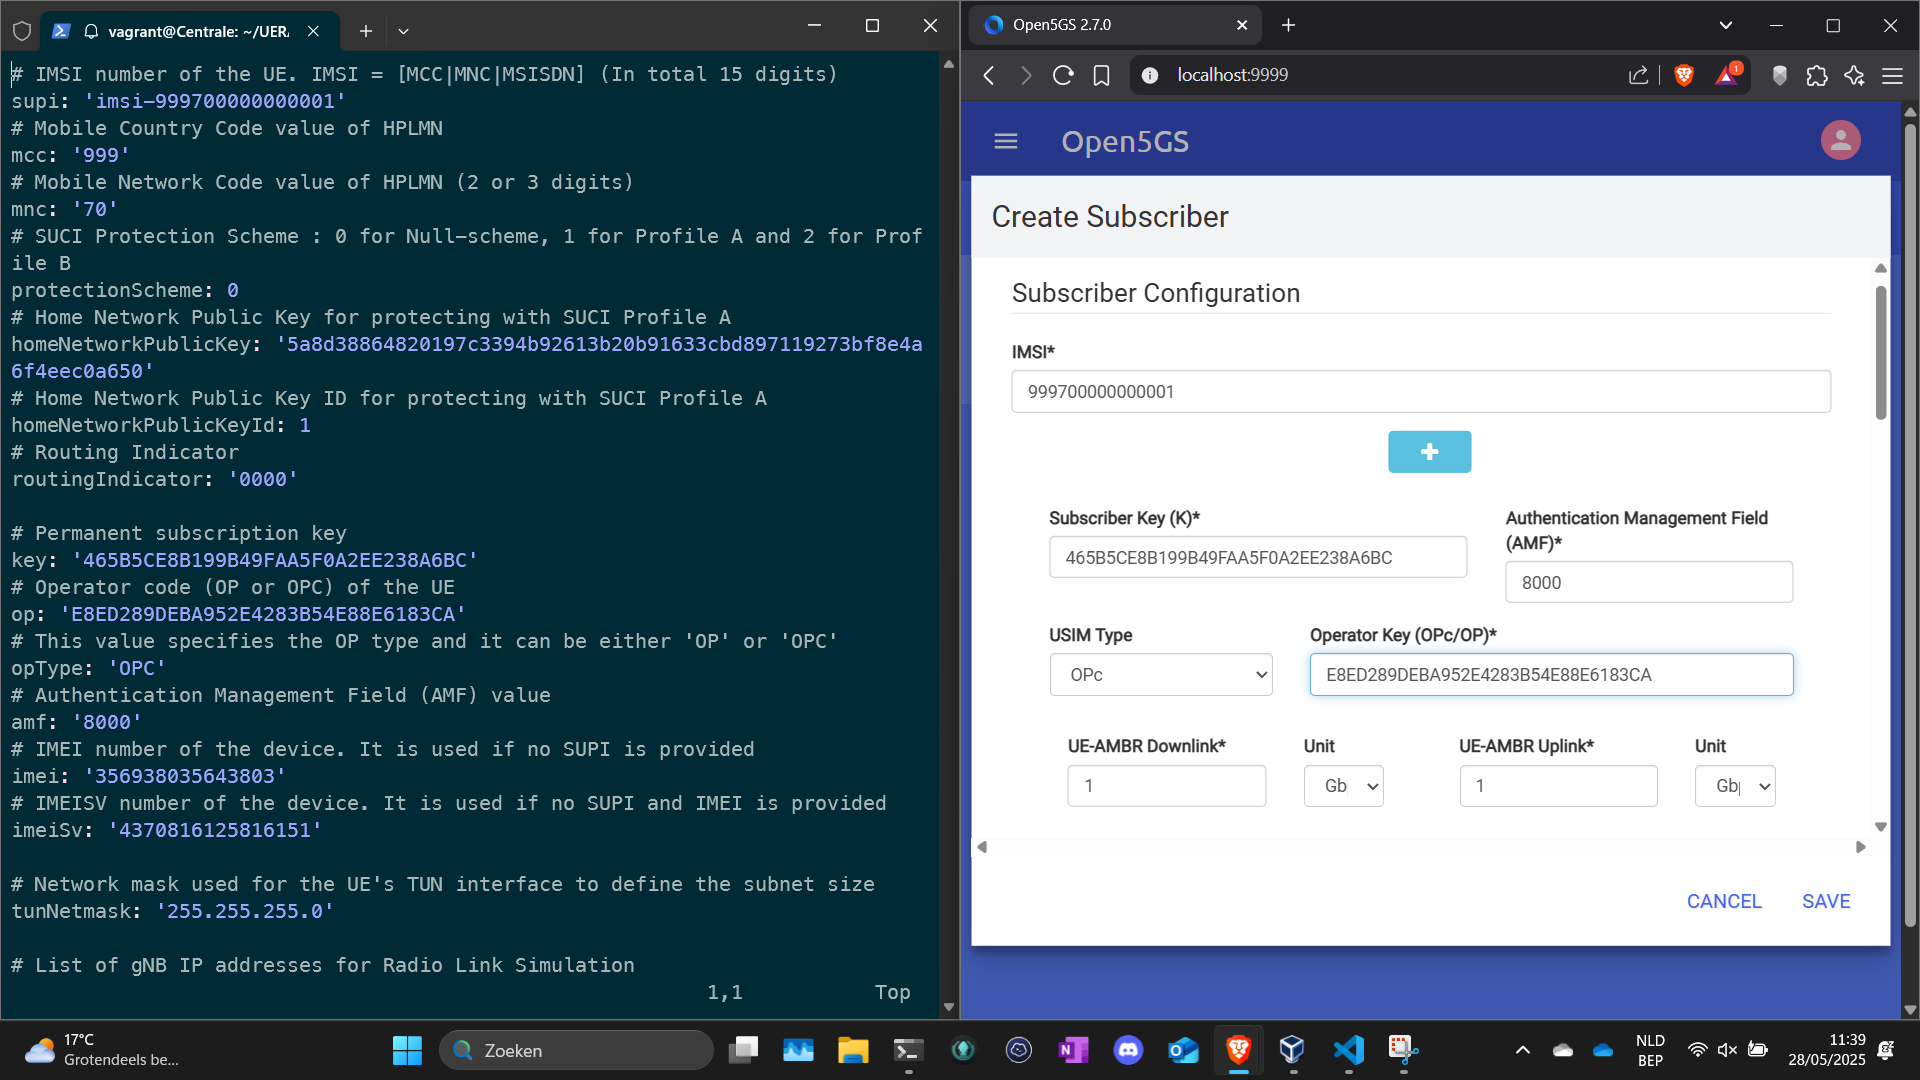
\includegraphics[width=\linewidth]{../graphics/POC-subConfig.png}
    \caption{Configuratie Subscriber (Screenshot)}
    \label{fig:SubConfig}
\end{figure}

Na de configuratie sla de subscriber op. Nu is het netwerk volledige geconfigureerd. 

\subsection{\IfLanguageName{dutch}{Run}{Run}}%
\label{sec:run}%

Om de simulatie te starten is het noodzakelijk om een 2de ssh sessie te openen.
In de eerste sessie start je de \gls{gnb} module. Dit wordt gestart aan de hand van de volgende commando's met hun corresponderende resultaat:

\begin{lstlisting}[basicstyle=\small, frame=single, breaklines=true, postbreak=\mbox{\textcolor{red}{$\hookrightarrow$}\space}, escapeinside ={\%,}, escapechar={!}, numbers=left, language=sh, caption=gNB run en resultaat]
cd ~/UERANSIM/build
vagrant@ue:~/UERANSIM/build$ ./nr-gnb -c ../config/open5gs-gnb.yaml

UERANSIM v3.2.7
[2025-05-29 10:23:08.261] [sctp] [info] Trying to establish SCTP connection... (10.0.0.10:38412)
[2025-05-29 10:23:08.343] [sctp] [info] SCTP connection established (10.0.0.10:38412)
[2025-05-29 10:23:08.343] [sctp] [debug] SCTP association setup ascId[3]
[2025-05-29 10:23:08.343] [ngap] [debug] Sending NG setup Request
[2025-05-29 10:23:08.349] [ngap] [debug] NG setup Response received
[2025-05-29 10:23:08.349] [ngap] [info] NG setup procedure is successful
[2025-05-29 10:23:59.177] [rrc] [debug] UE[1] new signal detected
[2025-05-29 10:23:59.179] [rrc] [info] RRC setup for UE[1]
[2025-05-29 10:23:59.180] [ngap] [debug] Initial NAS message received from UE[1]
[2025-05-29 10:23:59.207] [ngap] [debug] Initial Context setup Request received
[2025-05-29 10:23:59.439] [ngap] [info] PDU session resource(s) setup for UE[1] count[1]
[2025-05-29 10:24:04.086] [rls] [debug] UE[1] signal lost
[2025-05-29 10:24:05.848] [rrc] [debug] UE[2] new signal detected
[2025-05-29 10:24:05.850] [rrc] [info] RRC setup for UE[2]
[2025-05-29 10:24:05.851] [ngap] [debug] Initial NAS message received from UE[2]
[2025-05-29 10:24:05.867] [ngap] [debug] UE Context Release Command received
[2025-05-29 10:24:05.867] [rrc] [info] Releasing RRC connection for UE[1]
[2025-05-29 10:24:05.874] [ngap] [debug] Initial Context setup Request received
[2025-05-29 10:24:06.094] [ngap] [info] PDU session resource(s) setup for UE[2] count[1]
\end{lstlisting}

\begin{lstlisting}[basicstyle=\small, frame=single, breaklines=true, postbreak=\mbox{\textcolor{red}{$\hookrightarrow$}\space}, escapeinside ={\%,}, escapechar={!}, numbers=left, language=sh, caption=UE run en resultaat]
cd ~/UERANSIM/build
vagrant@Centrale:~/UERANSIM/build$ sudo ./nr-ue -c ../config/open5gs-ue.yaml

UERANSIM v3.2.7
[2025-05-29 08:05:17.683] [nas] [info] UE switches to state [MM-DEREGISTERED/PLMN-SEARCH]
[2025-05-29 08:05:17.685] [rrc] [debug] New signal detected for cell[1], total [1] cells in coverage
[2025-05-29 08:05:17.685] [nas] [info] Selected plmn[999/70]
[2025-05-29 08:05:17.685] [rrc] [info] Selected cell plmn[999/70] tac[1] category[SUITABLE]
[2025-05-29 08:05:17.685] [nas] [info] UE switches to state [MM-DEREGISTERED/PS]
[2025-05-29 08:05:17.685] [nas] [info] UE switches to state [MM-DEREGISTERED/NORMAL-SERVICE]
[2025-05-29 08:05:17.685] [nas] [debug] Initial registration required due to [MM-DEREG-NORMAL-SERVICE]
[2025-05-29 08:05:17.685] [nas] [debug] UAC access attempt is allowed for identity[0], category[MO_sig]
[2025-05-29 08:05:17.686] [nas] [debug] Sending Initial Registration
[2025-05-29 08:05:17.686] [nas] [info] UE switches to state [MM-REGISTER-INITIATED]
[2025-05-29 08:05:17.686] [rrc] [debug] Sending RRC setup Request
[2025-05-29 08:05:17.687] [rrc] [info] RRC connection established
[2025-05-29 08:05:17.688] [rrc] [info] UE switches to state [RRC-CONNECTED]
[2025-05-29 08:05:17.688] [nas] [info] UE switches to state [CM-CONNECTED]
[2025-05-29 08:05:17.697] [nas] [debug] Authentication Request received
[2025-05-29 08:05:17.697] [nas] [debug] Received SQN [000000000101]
[2025-05-29 08:05:17.697] [nas] [debug] SQN-MS [000000000000]
[2025-05-29 08:05:17.701] [nas] [debug] Security Mode Command received
[2025-05-29 08:05:17.702] [nas] [debug] Selected integrity[2] ciphering[0]
[2025-05-29 08:05:17.713] [nas] [debug] Registration accept received
[2025-05-29 08:05:17.713] [nas] [info] UE switches to state [MM-REGISTERED/NORMAL-SERVICE]
[2025-05-29 08:05:17.713] [nas] [debug] Sending Registration Complete
[2025-05-29 08:05:17.713] [nas] [info] Initial Registration is successful
[2025-05-29 08:05:17.713] [nas] [debug] Sending PDU Session Establishment Request
[2025-05-29 08:05:17.714] [nas] [debug] UAC access attempt is allowed for identity[0], category[MO_sig]
[2025-05-29 08:05:17.921] [nas] [debug] Configuration Update Command received
[2025-05-29 08:05:17.949] [nas] [debug] PDU Session Establishment Accept received
[2025-05-29 08:05:17.949] [nas] [info] PDU Session establishment is successful PSI[1]
[2025-05-29 08:05:17.969] [app] [info] Connection setup for PDU session[1] is successful, TUN interface[uesimtun0, 10.45.0.8] is up.
\end{lstlisting}

Hieronder twee screenshot met de volledige overview van de terminals.

\begin{figure}[H]
    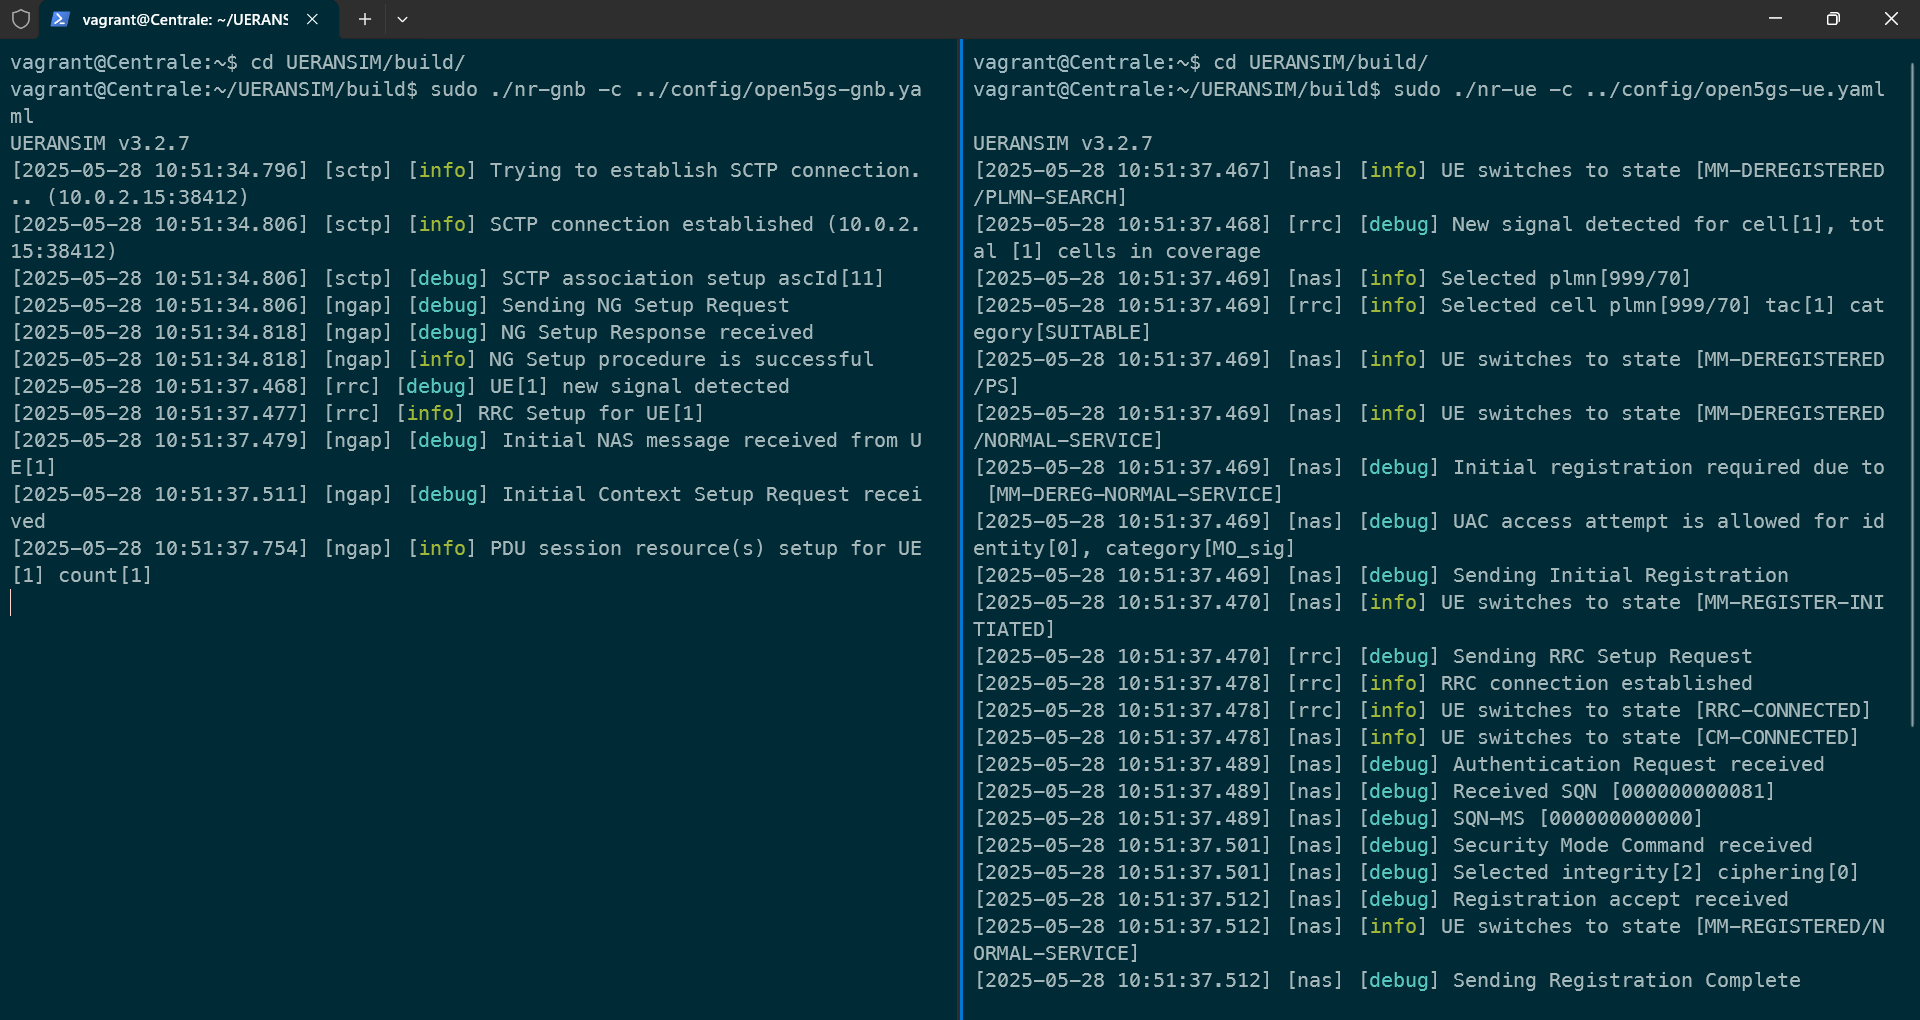
\includegraphics[width=\linewidth]{../graphics/POC-Run-1.png}
    \caption{Running the simulation (Part 1) (Screenshot)}
    \label{fig:runPart1}
\end{figure}
\begin{figure}[H]
    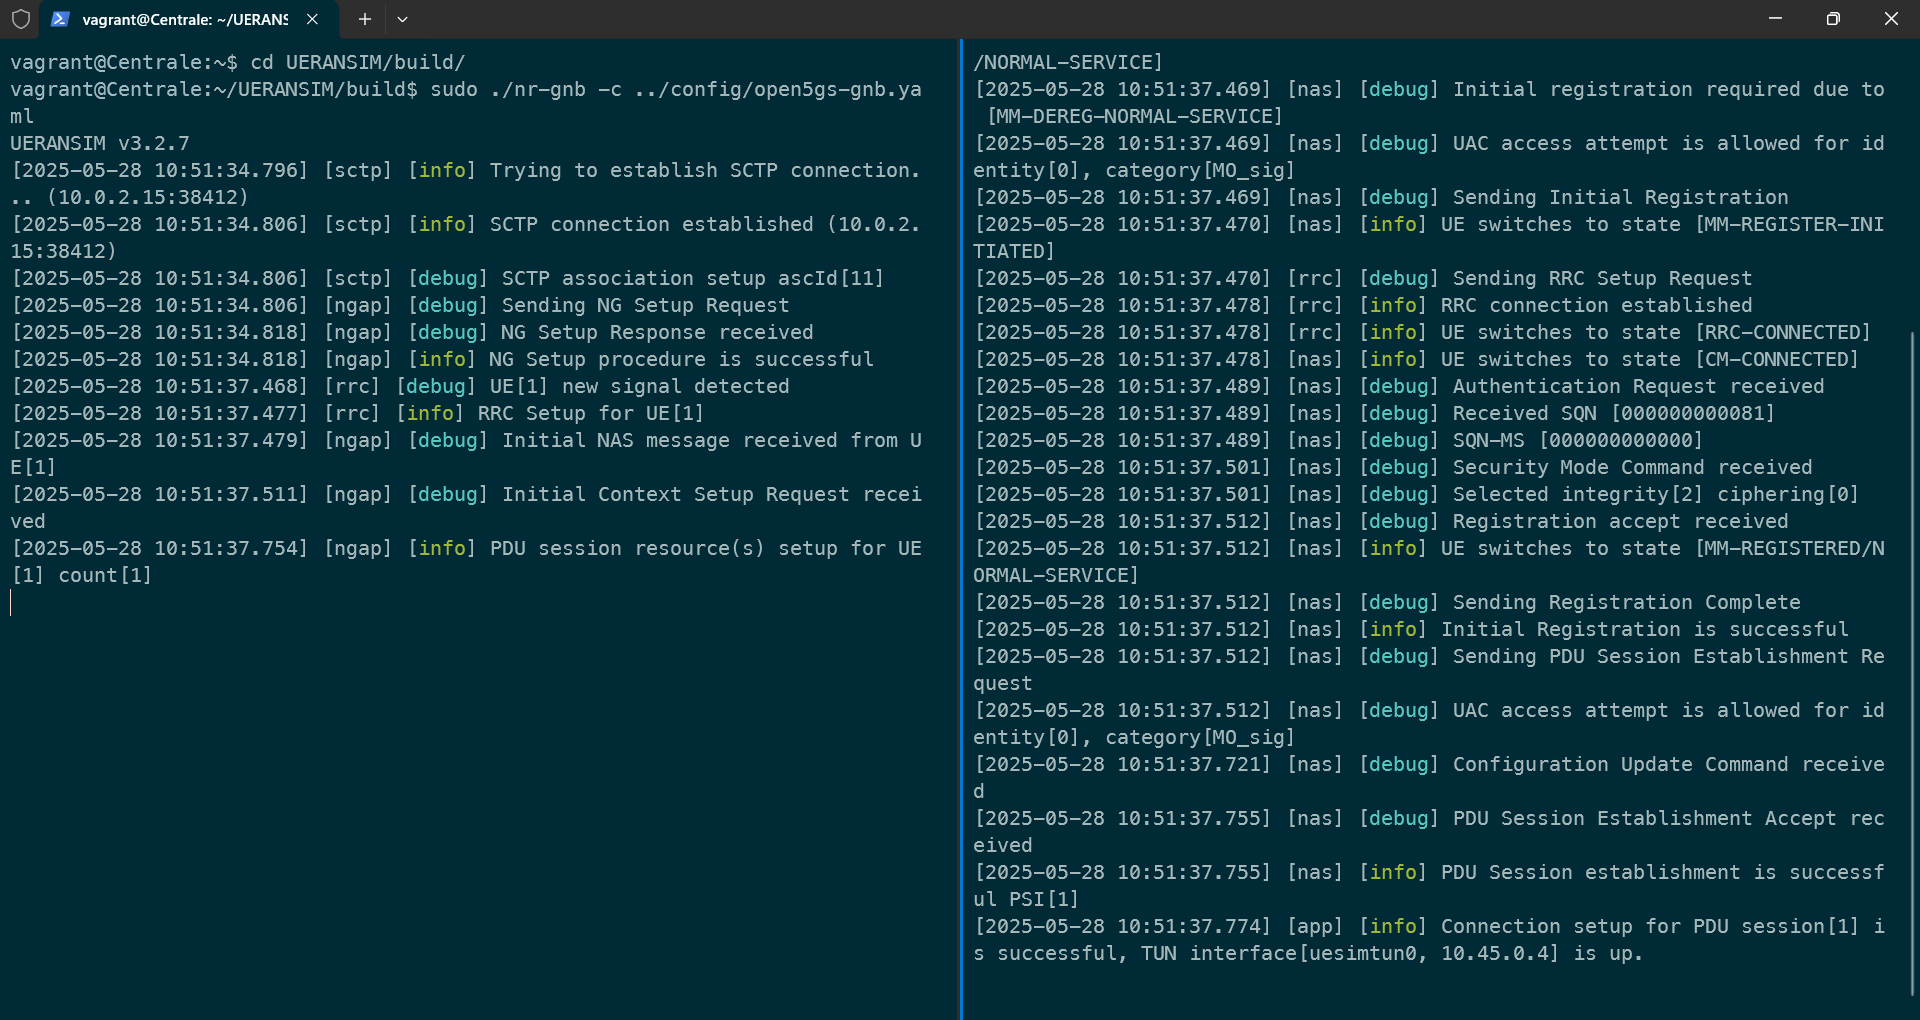
\includegraphics[width=\linewidth]{../graphics/POC-Run-2.png}
    \caption{Running the simulation (Part 2) (Screenshot)}
    \label{fig:runPart2}
\end{figure}

\section{\IfLanguageName{dutch}{Test}{Testing}}%
\label{sec:Test}%

\begin{figure}[H]
    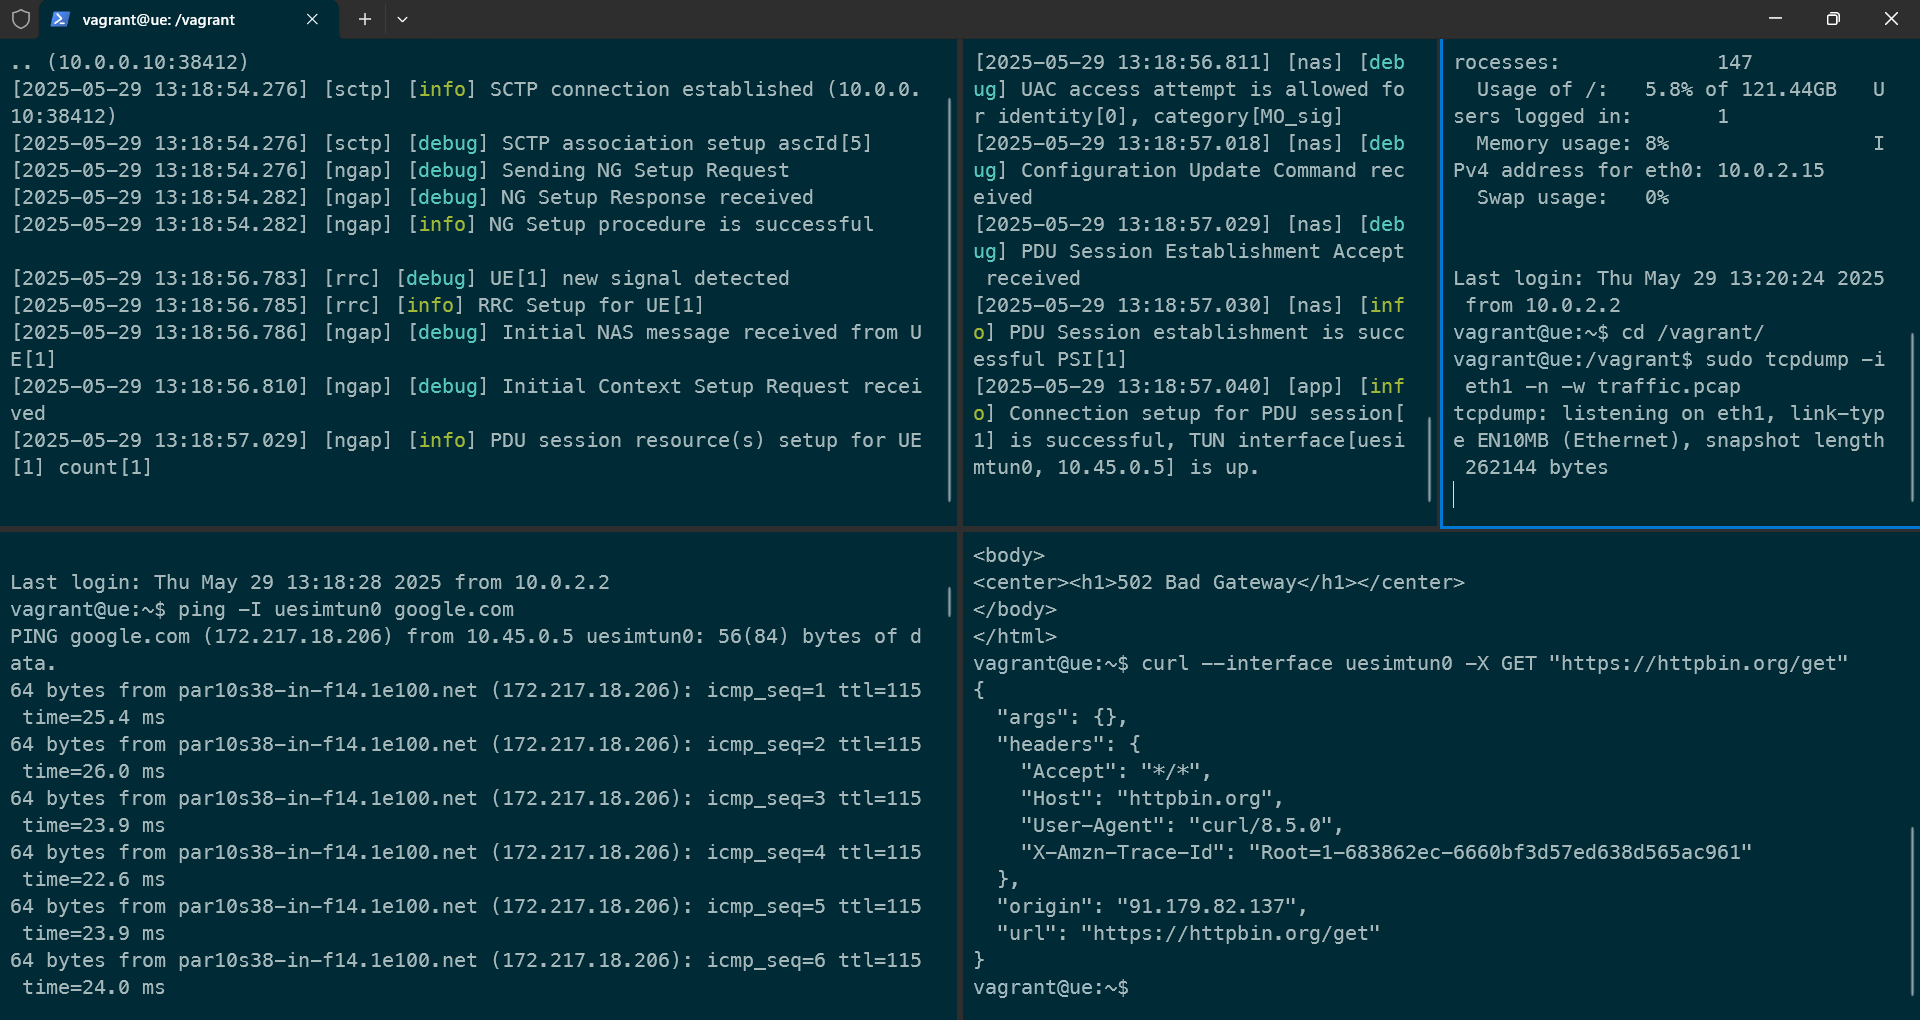
\includegraphics[width=\linewidth]{../graphics/POC-test.png}
    \caption{Testing (Screenshot)}
    \label{fig:Test-Overview}
\end{figure}

Om te controleren of de set-up is gelukt zijn er verschillende testen die kunnen worden uitgevoerd.

\begin{enumerate}
    \item Netwerkkaart
    \item Wireshark
    \item Ping
    \item Curl
\end{enumerate}

\subsection{\IfLanguageName{dutch}{Netwerkkaart}{network interface card}}%
\label{sec:Test-NIC}%

Er moet een nieuwe netwerkkaart verschijnen met naam \textbf{uesimtun0}.
Dit kan op 2 manieren worden gecontrolleerd.

De ene manier is via het commando \lstinline!ip a!.
\begin{lstlisting}[basicstyle=\small, frame=single, breaklines=true, postbreak=\mbox{\textcolor{red}{$\hookrightarrow$}\space}, escapeinside ={\%,}, escapechar={!}, numbers=left, language=sh, caption=Test - ip a]
vagrant@ue:~$ ip a
... 

7: uesimtun0: <POINTOPOINT,PROMISC,NOTRAILERS,UP,LOWER_UP> mtu 1400 qdisc fq_codel state UNKNOWN group default qlen 500
    link/none
    inet 10.45.0.6/24 scope global uesimtun0
       valid_lft forever preferred_lft forever
    inet6 fe80::d55b:6f3f:aa19:fcf7/64 scope link stable-privacy
       valid_lft forever preferred_lft forever
\end{lstlisting}


De andere manier is met het commando \lstinline!ifconfig!.
\begin{lstlisting}[basicstyle=\small, frame=single, breaklines=true, postbreak=\mbox{\textcolor{red}{$\hookrightarrow$}\space}, escapeinside ={\%,}, escapechar={!}, numbers=left, language=sh, caption=Test - ifconfig]
vagrant@ue:~$ ifconfig
...

uesimtun0: flags=369<UP,POINTOPOINT,NOTRAILERS,RUNNING,PROMISC>  mtu 1400
        inet 10.45.0.6  netmask 255.255.255.0  destination 10.45.0.6
        inet6 fe80::d55b:6f3f:aa19:fcf7  prefixlen 64  scopeid 0x20<link>
        unspec 00-00-00-00-00-00-00-00-00-00-00-00-00-00-00-00  txqueuelen 500  (UNSPEC)
        RX packets 0  bytes 0 (0.0 B)
        RX errors 0  dropped 0  overruns 0  frame 0
        TX packets 8  bytes 496 (496.0 B)
        TX errors 0  dropped 0 overruns 0  carrier 0  collisions 0
\end{lstlisting}

\subsection{\IfLanguageName{dutch}{Wireshark}{Wireshark}}%
\label{sec:Test-capture}%

Dit is een stap in het testplan dat blijft lopen tot de laatste stap is afgerond. Op deze manier wordt een optimale netwerk opname gegarandeerd. De opname wordt uitgevoerd vanuit de /vagrant directory. Dit is omdat dit de op voorhand geconfigureerde gedeelde map is. Door de netwerkopname hier uit te voeren, zorgen we ervoor dat de laptop ook aan de opname kan. Hierdoor kan een Wireshark GUI worden gebruikt.

\begin{lstlisting}[basicstyle=\small, frame=single, breaklines=true, postbreak=\mbox{\textcolor{red}{$\hookrightarrow$}\space}, escapeinside ={\%,}, escapechar={!}, numbers=left, language=sh, caption=Test - Tcpdump]
cd /vagrant/
sudo tcpdump -i eth1 -n -w traf.pcap
\end{lstlisting}

\begin{figure}[H]
    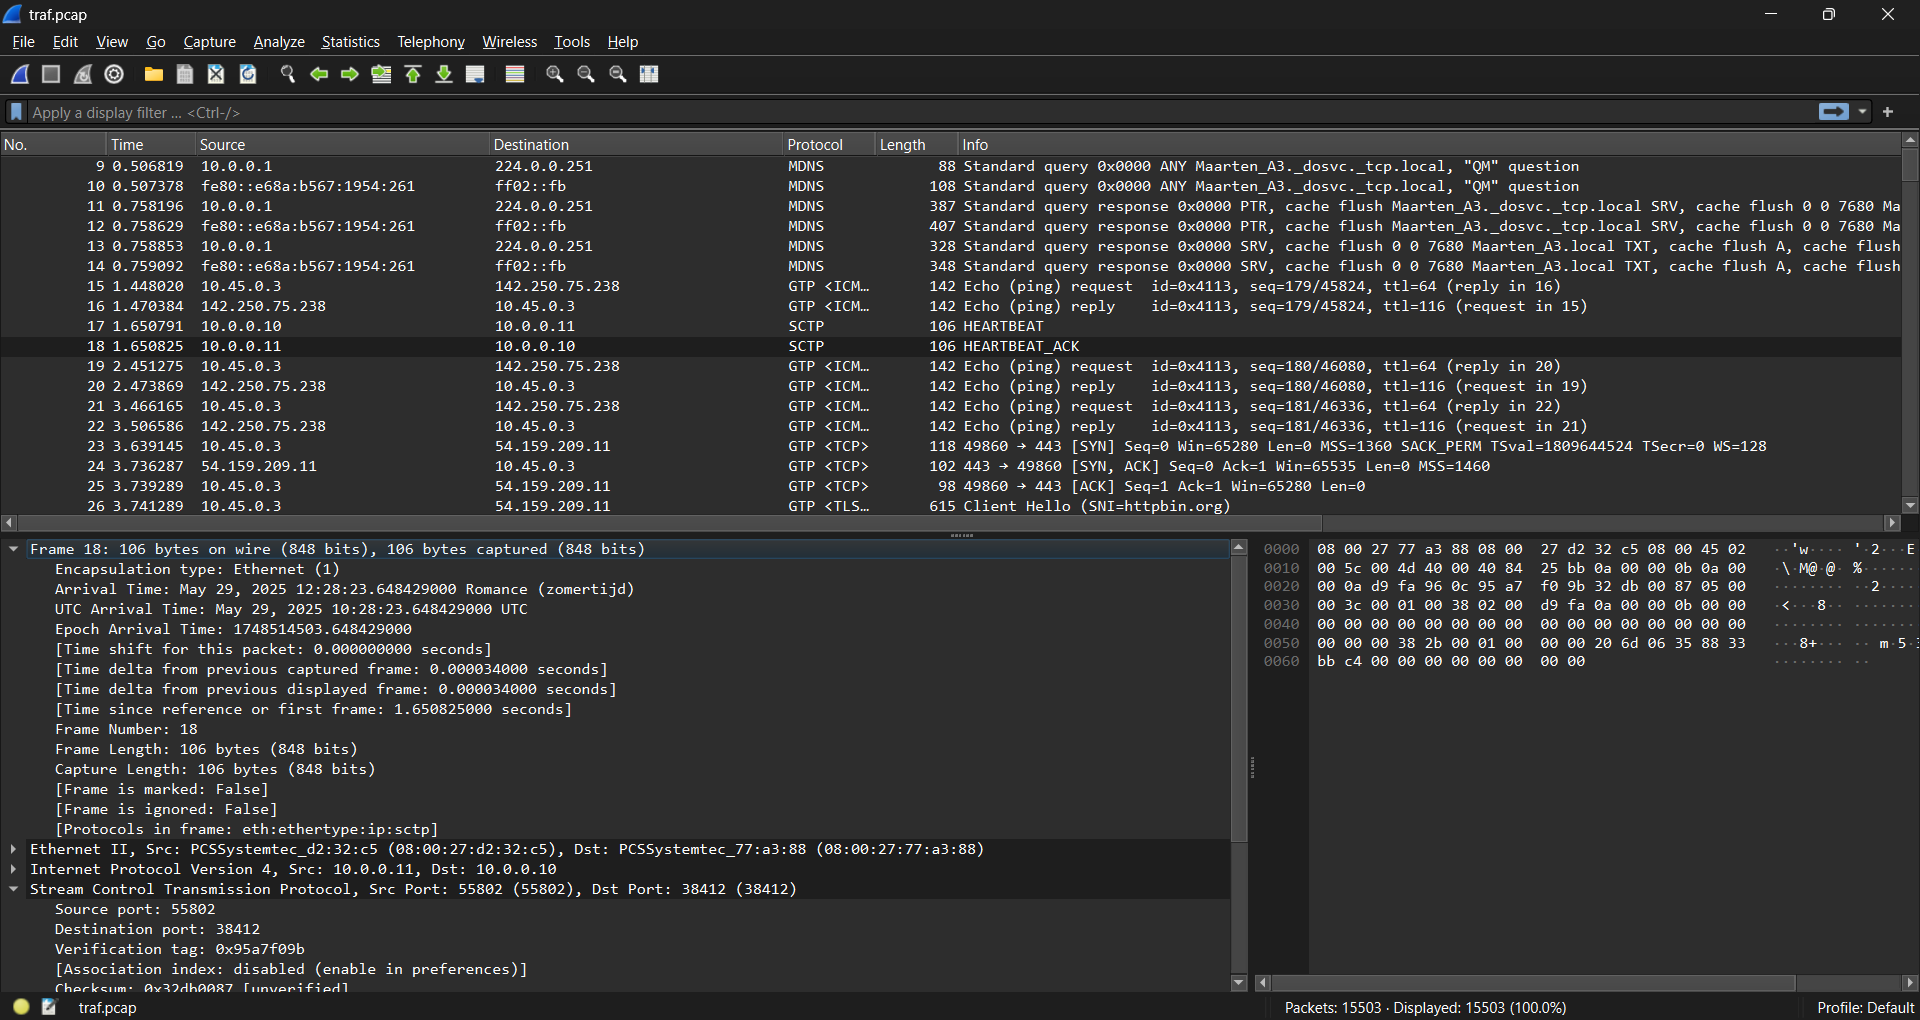
\includegraphics[width=\linewidth]{../graphics/POC-wireshark.png}
    \caption{Network capture in wireshark (Screenshot)}
    \label{fig:wireshark}
\end{figure}

In deze capture zijn er aan aantal zaken die duiden op een geslaagde run van het netwerk. Al deze steunen op hun type protocol dat is gecaptured.\\\\

De eerste is de packets van het protocol SCTP. Deze packets zijn voornamelijk heartbeats met corresponderende Acknowledgements. Dit is een controle op de 5G connectie tussen de \gls{ue} en de \gls{gnb}. Van zorda deze verschijnt en blijft terugkeren, kan men concluderen dat er een 5G connectie bestaat.\\


Het volgende protocol waarvan packtes zijn gecaptured, en dus een geslaagde netwerkopstelling aantoont, is de \gls{gtp} packets.
Dit is een tunnel protocol, dat wordt gebruikt vppr roaming, \gls{ran}, \gls{ciot} deployments en in packets van de core voor 3G, 4G en 5G netwerken. \autocite{palo2022} Dit is dus eeen soort van drager van packets die langs de core moeten passeren.\\\\
Dit is ook logisch aangezien de packets die hierin zitten TCP, TLS en ICMP packets zijn. Wat correspondeert met de protocollen van ping en curl. de andere 2 testen die werden uitgevoerd terwijl de netwerk opname werd gemaakt.
\subsection{\IfLanguageName{dutch}{Ping}{Ping}}%
\label{sec:Test-ping}%

\begin{lstlisting}[basicstyle=\small, frame=single, breaklines=true, postbreak=\mbox{\textcolor{red}{$\hookrightarrow$}\space}, escapeinside ={\%,}, escapechar={!}, numbers=left, language=sh, caption=Test - Ping]
    vagrant@ue:~$ ping -I uesimtun0 google.Com
PING google.Com (172.217.20.206) from 10.45.0.3 uesimtun0: 56(84) bytes of data.
64 bytes from par10s41-in-f14.1e100.net (142.250.75.238): icmp_seq=6182 ttl=116 time=25.1 ms
...
64 bytes from par10s41-in-f14.1e100.net (142.250.75.238): icmp_seq=6183 ttl=116 time=41.6 ms
64 bytes from par10s41-in-f14.1e100.net (142.250.75.238): icmp_seq=6184 ttl=116 time=30.3 ms
64 bytes from par10s41-in-f14.1e100.net (142.250.75.238): icmp_seq=6185 ttl=116 time=38.5 ms
64 bytes from par10s41-in-f14.1e100.net (142.250.75.238): icmp_seq=6186 ttl=116 time=23.5 ms
...
--- google.Com ping statistics ---
6198 packets transmitted, 6195 received, 0.0484027% packet loss, time 6231019ms
rtt min/avg/max/mdev = 21.394/27.963/159.611/7.694 ms
vagrant@ue:~$
\end{lstlisting}

\subsection{\IfLanguageName{dutch}{Curl}{Curl}}%
\label{sec:Test-curl}%


\begin{lstlisting}[basicstyle=\small, frame=single, breaklines=true, postbreak=\mbox{\textcolor{red}{$\hookrightarrow$}\space}, escapeinside ={\%,}, escapechar={!}, numbers=left, language=sh, caption=Test - Curl]
vagrant@ue:~$ curl --interface uesimtun0 -X GET "https://httpbin.org/get"
{
  "args": {},
  "headers": {
    "Accept": "*/*",
    "Host": "httpbin.org",
    "User-Agent": "curl/8.5.0",
    "X-Amzn-Trace-Id": "Root=1-683836c9-7cca29e43a4cd009264470d9"
  },
  "origin": "91.179.82.137",
  "url": "https://httpbin.org/get"
}
\end{lstlisting}

Na deze controle wordt de netwerkopname stopgezet.

\section{\IfLanguageName{dutch}{Praktische integratie}{Possible practical integration}}%
\label{sec:integration}%

Een \'{e}\'{e}n-op-\'{e}\'{e}n conversie, op de manier zoals deze is geconfigureerd in de simulatie is mits de vereiste hardware zeker mogelijk. Echter van zodra men wil kijken naar slicing stoot men op problemen, zoals aangehaald in hoofdstuk \ref{sec:Slicing}. In de simulatie is dit een paar extra variabelen aanpassen bij de \gls{ue}. Zie de screenshot hieronder.


\begin{figure}[H]
    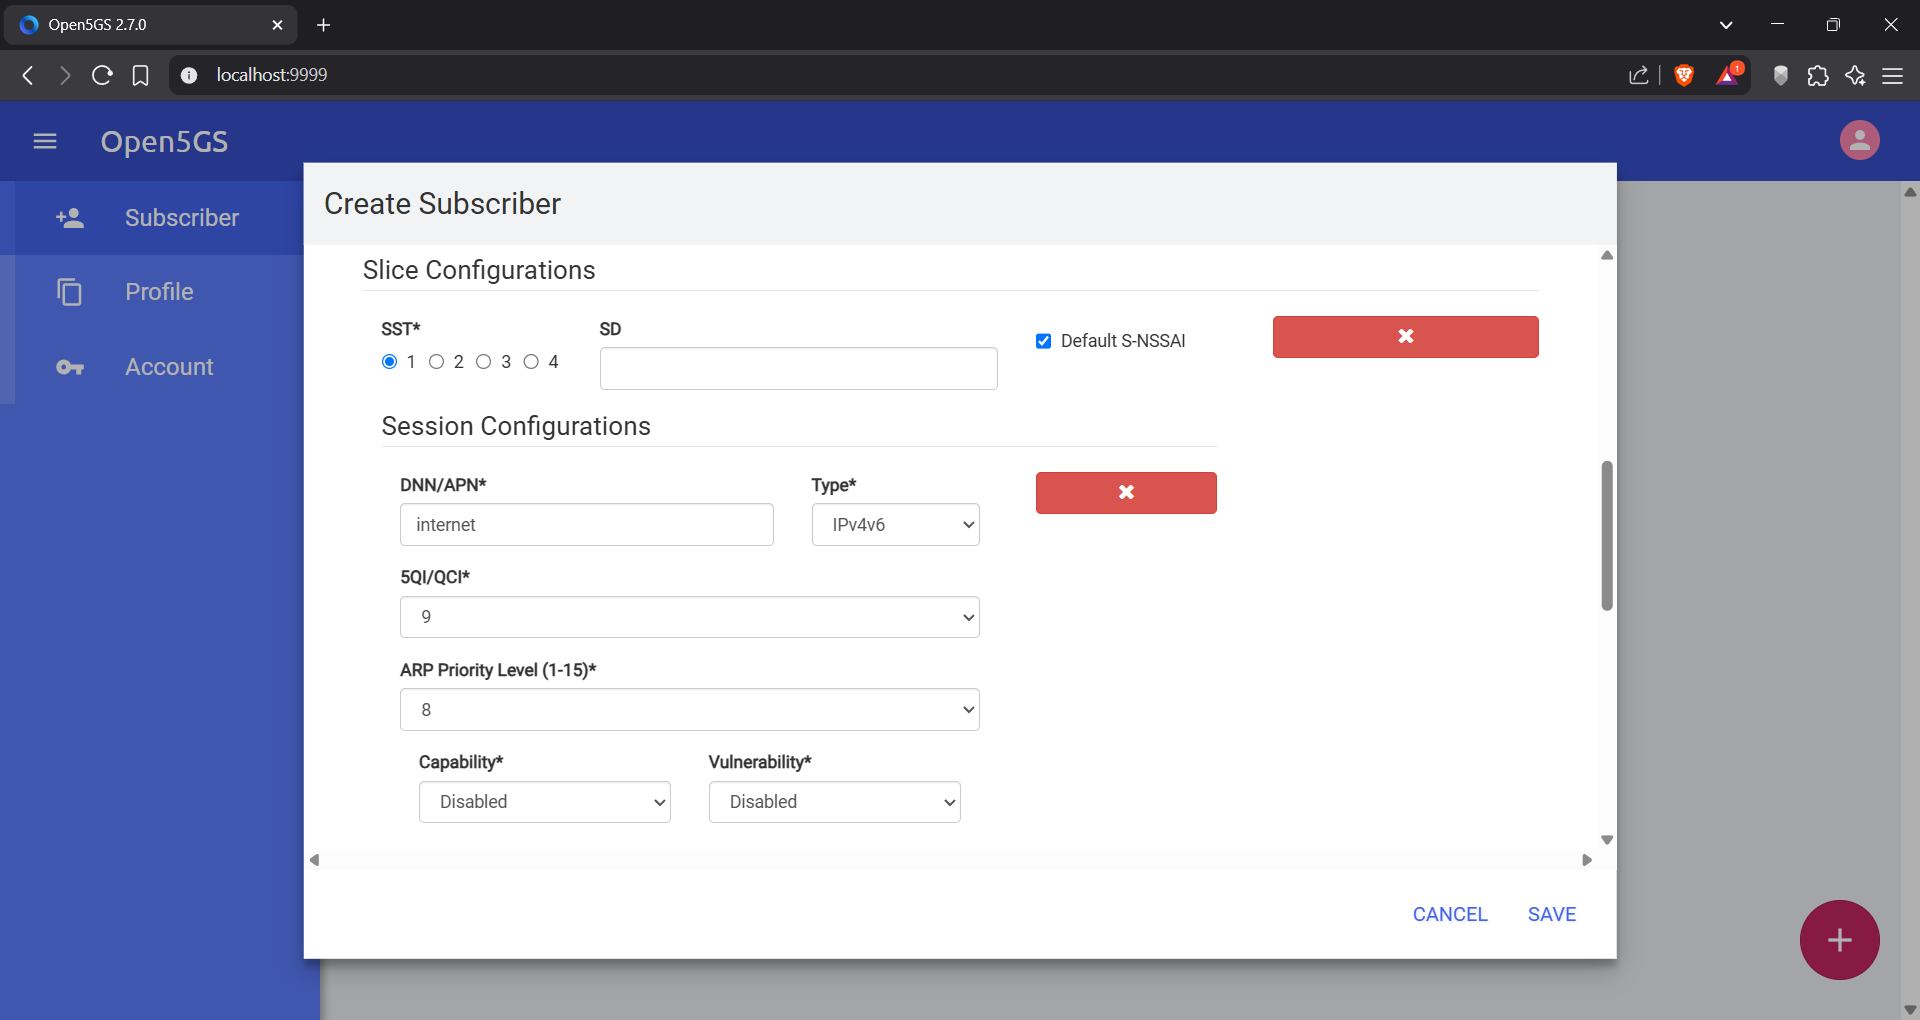
\includegraphics[width=\linewidth]{../graphics/POC-Slicing.png}
    \caption{PoC Slicing (Screenshot)}
    \label{fig:pocSlicing}
\end{figure}

% %TODO: Zebra TC27 Handheld Computer en conversie problemen?